\section{Les chaînes de Markov}
% Un algorithme de calcul de distance permet de mesurer la similarité et/ou la dif-
% férence entre deux objets tels que du texte, des vecteurs, des chaînes de caractères.
% On utilise ces algorithmes de calcul principalement pour la correction d’orthographe,
% le traitement de texte, les alignements de séquences ADN ou encore pour la recherche
% d’information


\begin{frame}{Définition d'une chaîne de Markov}
	\begin{itemize}
		\item \textbf{Chaîne de Markov} : Modèle mathématique représentant un système de probabilité. Les probabilités de passer d'un état à un autre dépendent entièrement de l'état actuel.
		\item \textbf{Etats} : Elements du système.
		\item \textbf{Transition} : Action de passer d'un état à un autre.
		\item \textbf{Matrice transition} : Table permettant de regrouper les transitions entre tous les états.
	\end{itemize}
	\begin{center}
		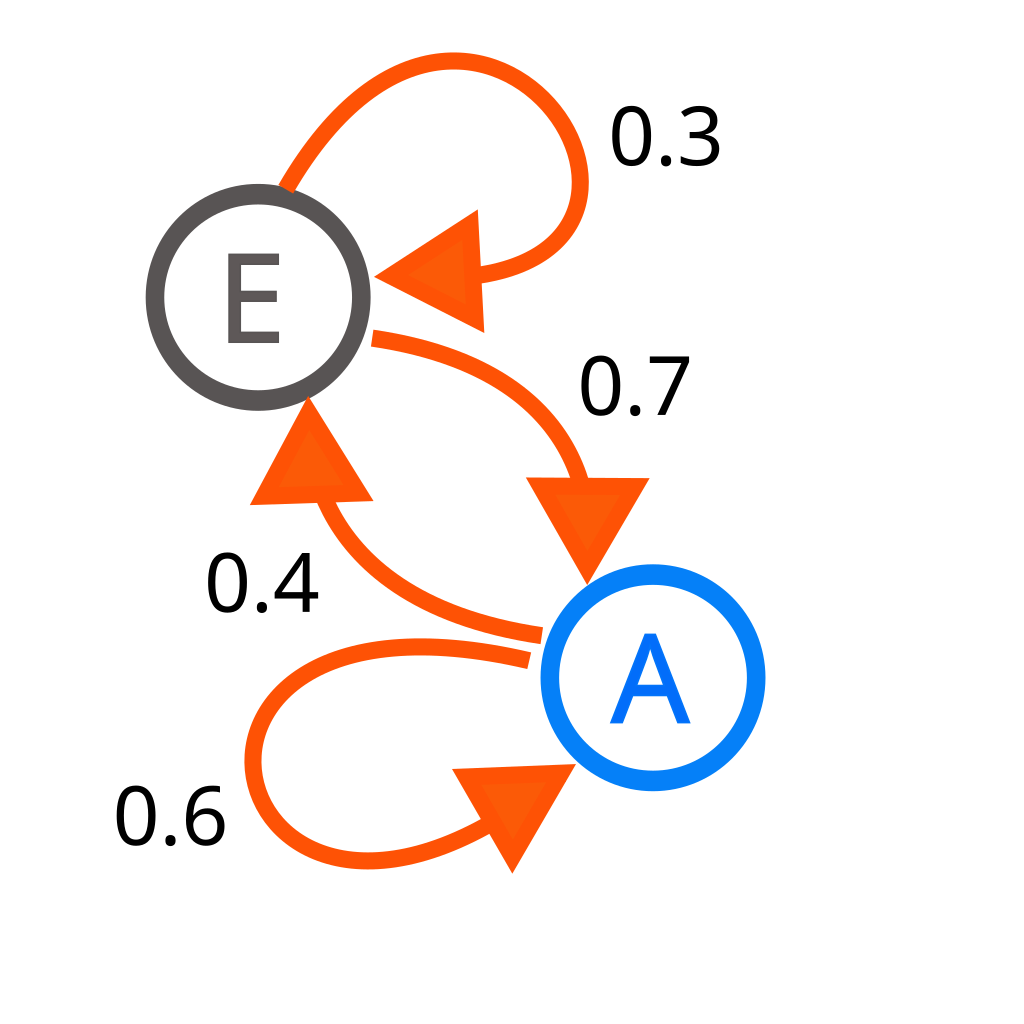
\includegraphics[width=0.38\textwidth]{images/def_markov.png}
		\vspace*{0.3cm}
	\end{center}

\end{frame}

\begin{frame}{Application}
	\vspace*{-0.3cm}
	Utilisation pour modélisation de processus aléatoires, analyse de séquences, de prédictions ou d'historiques de navigation.
	Analyse des historiques de navigation ainsi que les actions de l'utilisateur.

	\begin{center}
		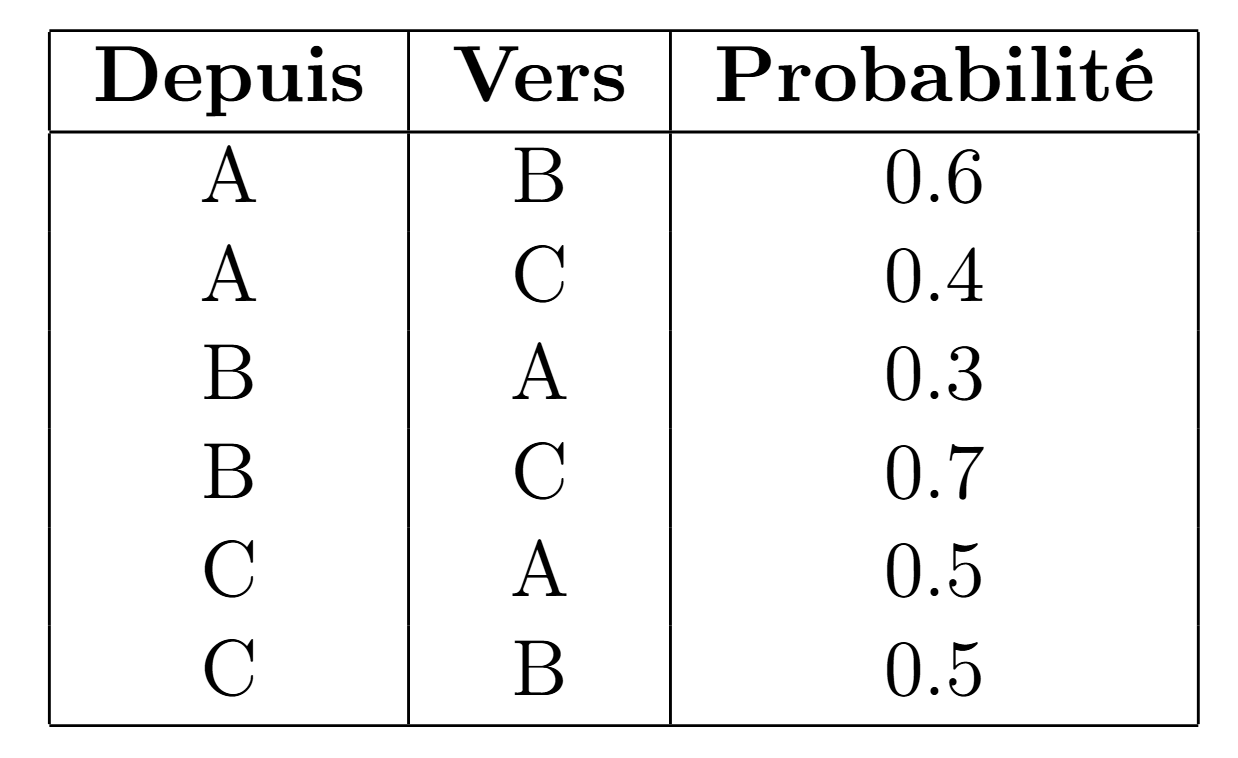
\includegraphics[width=0.6\textwidth]{images/tableau_proba_markov.png}
		\par
		Exemple transitions entre trois pages web A, B et C.
	\end{center}
\end{frame}

\begin{frame}{Matrice transition}
	Modélisation des transitions probables entre les étapes.
	\begin{itemize}
		\item Collecter les données
		\item Compter les transitions
		\item Calcul des probabilités
		\item Construction de la matrice
	\end{itemize}
	\begin{center}
		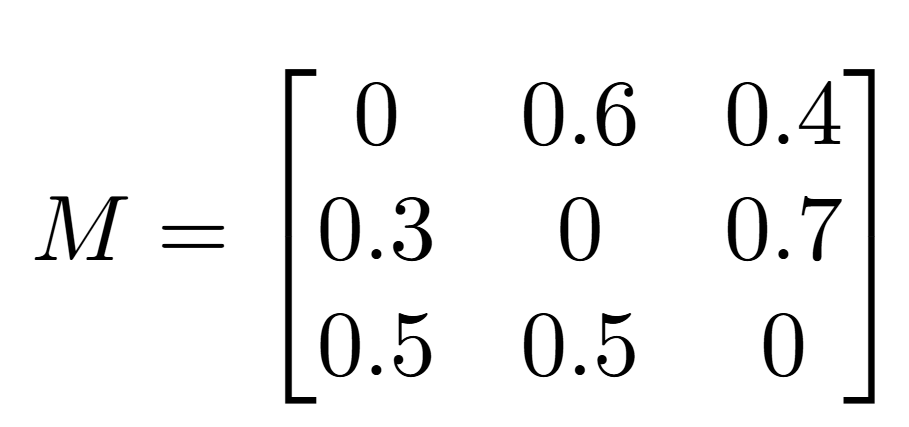
\includegraphics[width=0.6\textwidth]{images/matrice_transition.png}
		\par
		Resultat selon le tableau précédent
	\end{center}
\end{frame}

\begin{frame}{Exemple complet}
	\vspace{-0.5cm}
	\centering
	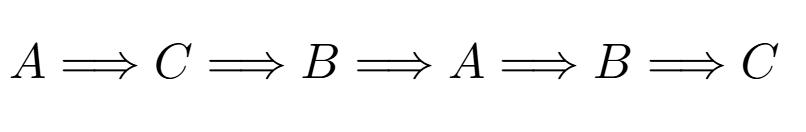
\includegraphics[width=0.8\textwidth]{images/transition_ex_markov.png}
	\vspace{1cm}
	\begin{columns}
		\column{0.6\textwidth}
		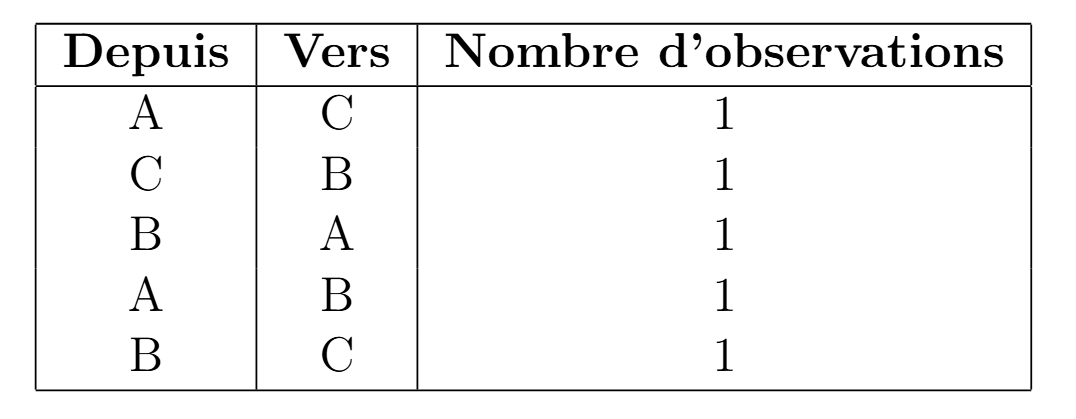
\includegraphics[width=\textwidth]{images/tableau_ex_markov.png}
		\column{0.4\textwidth}
		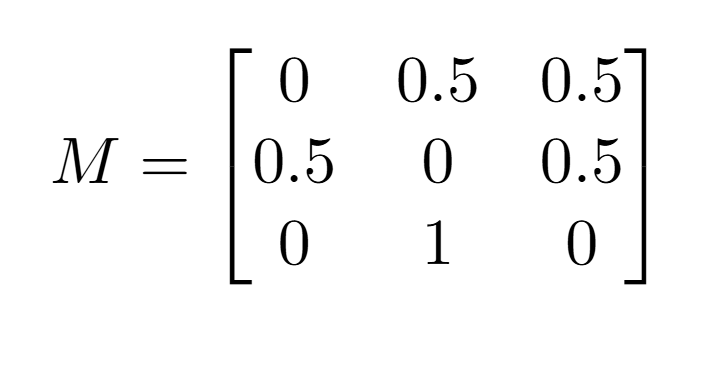
\includegraphics[width=\textwidth]{images/matrice_markov.png}
	\end{columns}
	\vspace{1cm}
	\textbf{Calcul probabilités} :  nombre de fois où la transition\(X\) vers \(Y\) est observée, puis de diviser par le total des transitions partant de l'état \(X\).
\end{frame}
